\section{Methods}

\subsection{Network notations}
A network is a mathematical object composed of a set of vertices (in ecology, it often represents individuals or genes) that are connected by edges representing their interactions.
Let's consider a location and the resulting interactions of this sampling. We consider a bipartite network, meaning that the vertices can be divided into two disjoint ensembles of vertices $R$ and $C$ with $r$ resource species and $c$ consumer species, with no intra-group interactions. In this case, the resources and consumers do not imply a predation. It can be plant/pollinators, host/parasites, or others as long as the network is bipartite.  All these interactions will be recorded in a two-way contingency matrix.



\subsection{Correspondence analysis} {\label{CA}}


Correspondence analysis (CA) \citep{hill_correspondence_1974, beh_simple_2004}, also known as reciprocal averaging is a multivariate statistical technique primarily developed to analyze two-way contingency tables (for example counting the eye color's distribution against the hair color for a set of individuals). It enables us to visualize the table in a lower dimensional space and put in evidence the relationship between the rows and the columns of the table.

It can be viewed as a three-step process. The first is obtaining the standardized residuals by computing the distances to the null (independence) model. The second one uses Singular Value Decomposition (SVD) to get the axes containing the maximum variance. Finally, we select the axes holding the most information to reduce the dimensionality of the data and visualize these components in a lower dimensionality space using the coordinates obtained with the singular value decomposition.


Let's consider a $r \times c$ two-way contingency matrix $\mathbf{Y} = [y_{ij}]$ such that $r\geq c$ and with $y_{ij}$ the number of observed interactions between species $i$ and $j$. Let $\mathbf{P}$ be the matrix of relative proportions $
\mathbf{P} = \left[ y_{ij} / \sum_{i=1}^{r} \sum_{j=1}^{c} y_{ij} \right]
$

The relative (or marginal) weights are computed as the column and row sums of the table $\mathbf{P}$: 
$$
    \mathbf{w}_r = \mathbf{P1_r}=\left[ p_{1+}, \dots, p_{r+}\right]^\top \quad \text{and} \quad \mathbf{w}_r = \mathbf{P}^\top \mathbf{1_c} = \left[ p_{+ 1}, \dots, p_{+ c}\right]^\top
$$

with $p_{+j} = \sum_ip_{ij}$ and $p_{i+} = \sum_jp_{ij}$ and $\mathbf{1}$ is a vector of ones of appropriate dimension. These weights are then transformed into diagonal matrices: 
$$
    \mathbf{W}_r = \text{diag}\left(\mathbf{w}_r\right) \quad \text{and} \quad \mathbf{W}_c = \text{diag}\left( \mathbf{w}_c \right)
$$

\subsubsection{Contribution to $\chi^2$ / distance to null model} \label{abund_effect_ca}

Let $\mathbf{P}_0$ be the $r\times c$ expected matrix under the null hypothesis that no relationship exists between the rows and the columns. We define $\mathbf{P}_0$ as:
$$
    \mathbf{P}_0 = \mathbf{w}_r \mathbf{w}_c^\intercal
$$

The Pearsons 's standardized residuals (that measures the departure of observations from random distribution) are then computed as $\mathbf{S} = \mathbf{W}_r^{-1/2} (\mathbf{P} - \mathbf{P}_0) \mathbf{W}_c^{-1/2}$

\subsubsection{Single Value Decomposition}

Singular value decomposition (SVD) is a generalization of the eigen-decomposition to rectangular matrices. It is widely used in fields like informatics for applications such as image compression. It enables the decomposition of the matrix into a sum of axes weighted by singular values, indicating the variance explained by each axis.

SVD enables the decomposition of a matrix such as the previous one under the form: 
$$
    \mathbf{S} = \mathbf{U}_{(r\times c)} \mathbf{\Sigma}_{(diagonal, c\times c)} \mathbf{V}_{(c \times c)}^\intercal \Leftrightarrow \mathbf{S} = \sum_i \sigma_i \mathbf{U}_i \mathbf{V}_i^\intercal
$$

\begin{figure}[h]
    \centering
    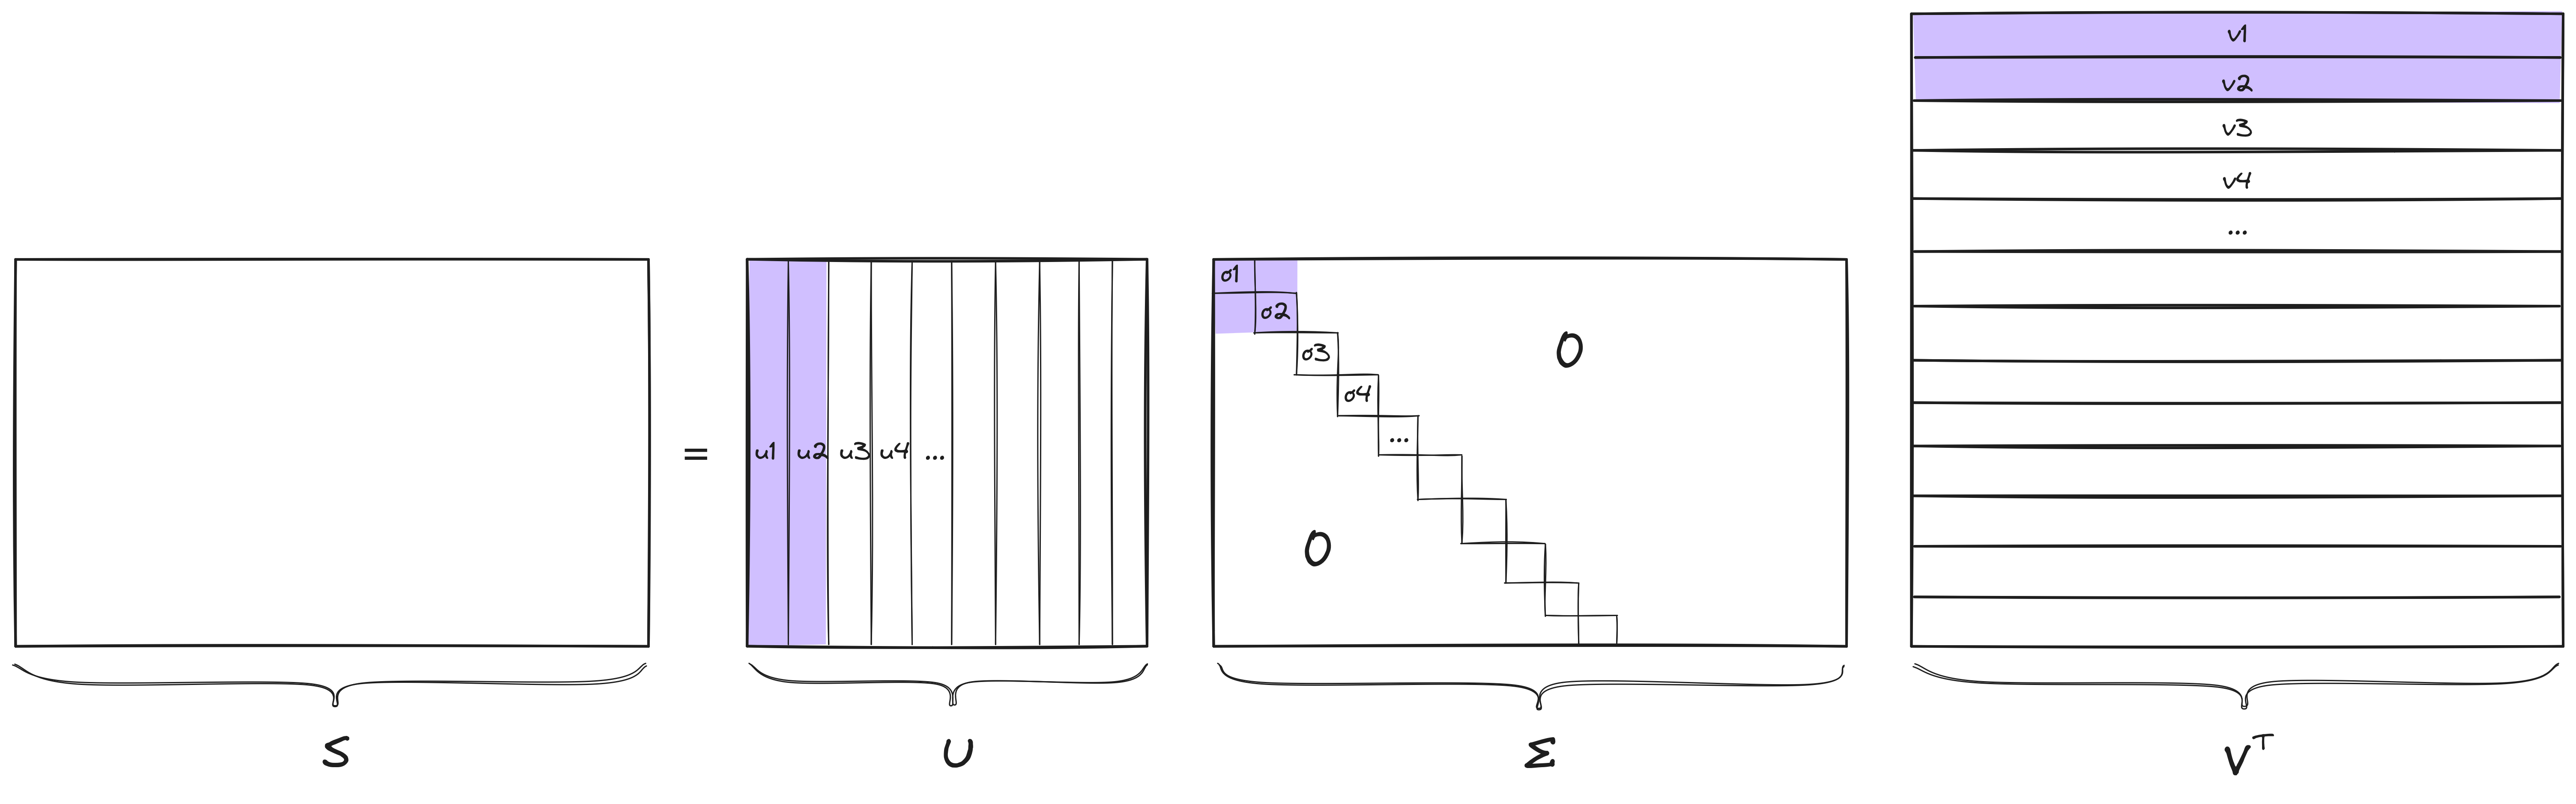
\includegraphics[width=1\linewidth]{FIGURES//methods/SVD.png}
    \caption{Visual representation of the SVD}
    \label{fig:SVD}
\end{figure}

where:
\begin{itemize}
    \item $\mathbf{U}$ and $\mathbf{V}$ are orthonormal left and right singular vectors such as $\mathbf{U}^\intercal\mathbf{U} = \mathbf{V}^\intercal\mathbf{V} = \mathbf{I}$.
    \item  $\mathbf{\Sigma}$ is a diagonal matrix $\mathbf{D}_{\sigma_i}$ with $\sigma_i \in \mathbb{R}^+$, which are the singular values of $\mathbf{S}$.
\end{itemize}


\paragraph{3: Coordinates}

To visualize the result, an additional step is needed to transform the singular vectors into coordinates that preserve the $\chi^2$ distances. The principal coordinates for the rows of $\mathbf{P}$ are computed as :
$$
    \mathbf{F}_r = \mathbf{W}_r^{-1/2} \mathbf{U} \mathbf{\Sigma}
$$
Similarly, the principal coordinates for the columns are computed as:
$$
    \mathbf{F}_c = \mathbf{W}_c^{-1/2} \mathbf{V} \mathbf{\Sigma}
$$ 


\subsection{Foucart Correspondence analysis}

Foucart Correspondence Analysis (also called Foucart COA) is a method used to analyze a series of contingency tables  crossing the same two variables (in our case consumers and resources) \citep{pavoine_new_2007}.
It is divided into two steps (Figure \ref{fig:foucart}), first Foucart COA aims to identify the common structure (associations between rows and columns that are present in all tables) and then the intra-structure of each contingency table (i.e., the variation of each table around the common structure).

Let be $\mathbf{Y}_1, \ldots, \mathbf{Y}_k, \ldots, \mathbf{Y}_K$ be $K$ contingency tables with the same $R$ rows and $C$ columns: $\mathbf{Y}_k = [y_{ij}^k]$. 
For each table $\mathbf{Y}_k$, we can define the matrix of relative frequencies $\mathbf{P}_k$ and $\mathbf{W}_r^k$ and $\mathbf{W}_r^k$, the associated diagonal matrices of row and column weights. Computations are presented in the \ref{CA} section 

\begin{figure}[h]
    \centering
    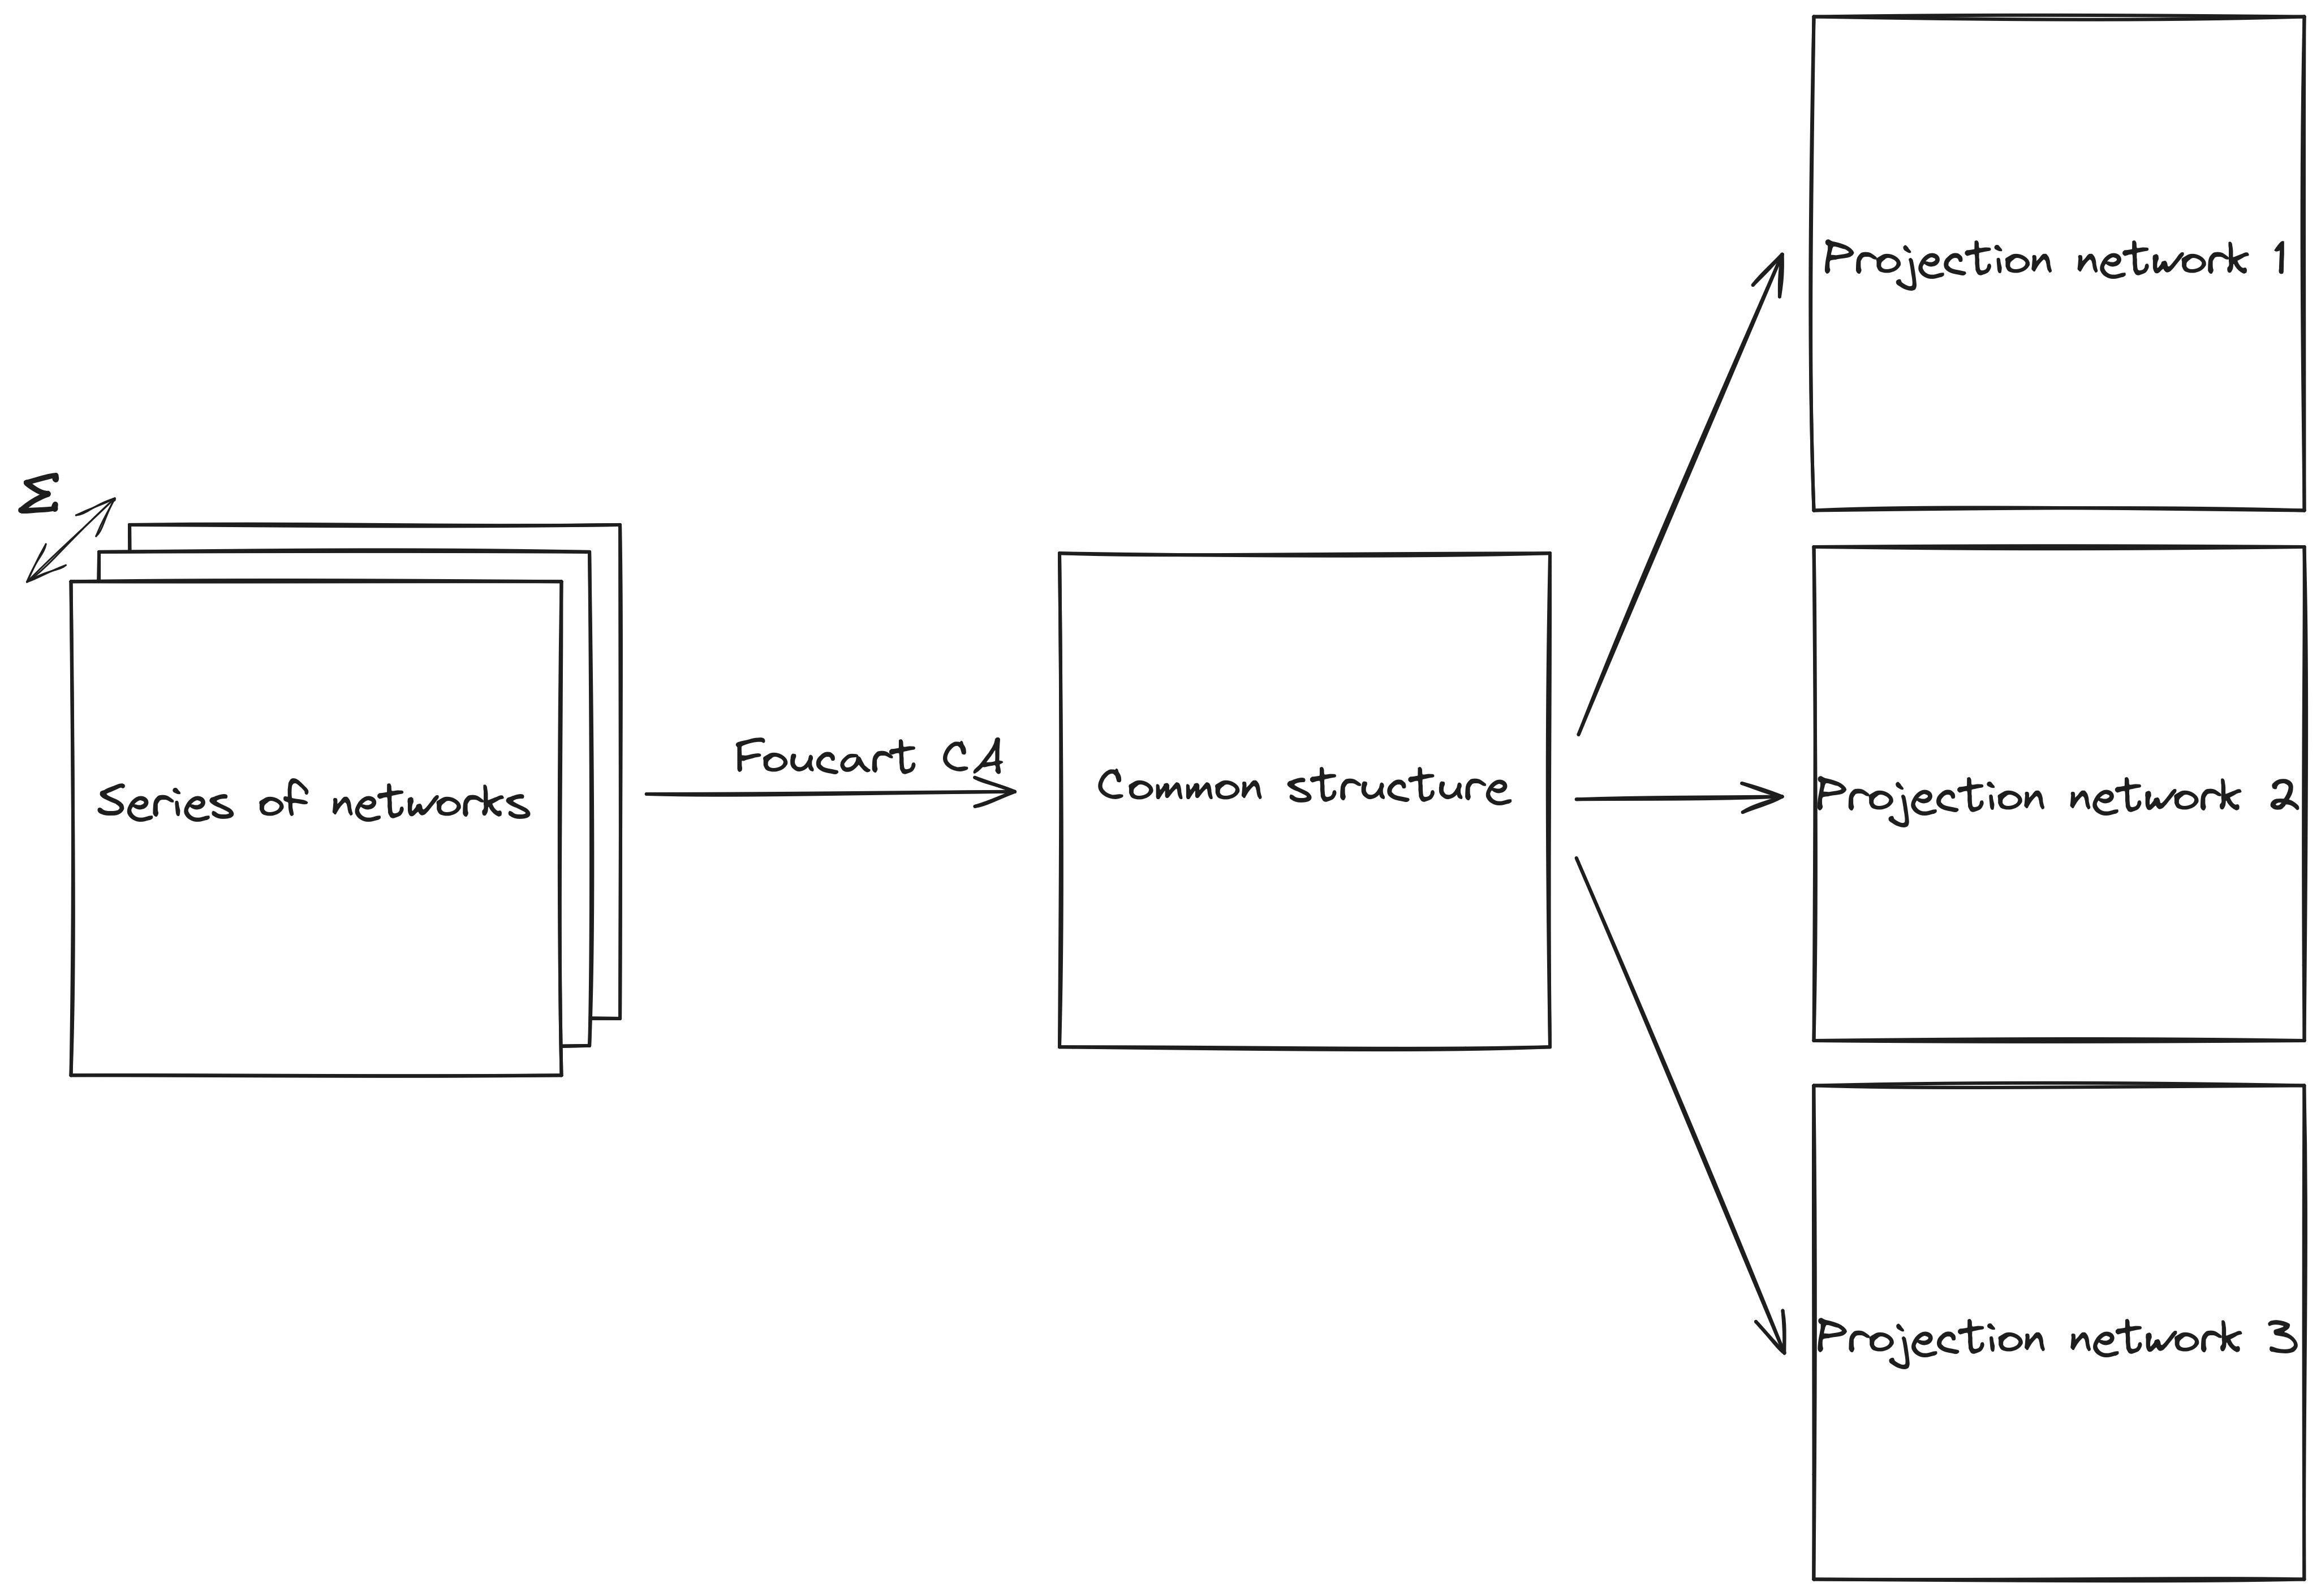
\includegraphics[width=0.75\linewidth]{FIGURES//methods/foucart.png}
    \caption{Visualization of Foucart CA}
    \label{fig:foucart}
\end{figure}

\subsubsection{Common structure}

In the first step, Foucart COA computes a regular CA on a common table computed as the sum of the contingency tables. We define the common table $\mathbf{P}$ as:
$$
    \mathbf{P} = \frac{1}{K} \sum_{k=1}^K \mathbf{P}^k = \left[ \frac{1}{K}\sum_{k=1}^{K}\frac{y_{ij}^k}{\sum_{i=1}^{r} \sum_{j=1}^{c} y_{ij}^k} \right]
$$
and then compute the CA on the matrix $\mathbf{P}$. This analysis produces the singular vectors $\mathbf{U}$ and $\mathbf{V}$.

\subsubsection{Intra-structure}

Next, we project the rows and columns of each individual contingency table onto the axes of the analysis of the common table.

$\mathbf{A} = c_1$ ce qui correspond à $\mathbf{F}_m$ ?
$\mathbf{B} = l_1$ ce qui correspond à $\mathbf{F}_n$ ?

The  projection of the columns is obtained by: $\left( \mathbf{P}^k (\mathbf{W}_c^k)^{-1} \right)^\intercal\mathbf{U}$
The projection of the rows is obtained by: $\left( (\mathbf{W}_r^k)^{-1}\mathbf{P}^k \right) \mathbf{V}$


\subsection{Bipartite network simulation}

Realistic interaction network generation is a complex task and many ways exist to generate some such as random geometric graphs or dendritic networks. We must fully know the input used to create and generate many networks to validate the method.

The simulation framework is based on Lisa Nicvert's thesis \citep{these_lisa_2024}, itself based on \cite{frund_sampling_2016}, \cite{benadi_quantitative_2022} and \cite{dray_testing_2008}.

For the simulation, we assume that the interactions are solely based on a mixed effect of the trait matching and the abundance. We can understand this as the probability of two species encountering, which is the product of the abundance, times the probability of these two species interacting together based on their trait matching.

Also, using a bipartite network assumes that there is no intra-group interaction but only inter-group interactions, meaning that competition, facilitation, and spatial exclusion will not be taken into account.

The simulation's steps will be depicted in the following sections

\begin{figure}
    \centering
    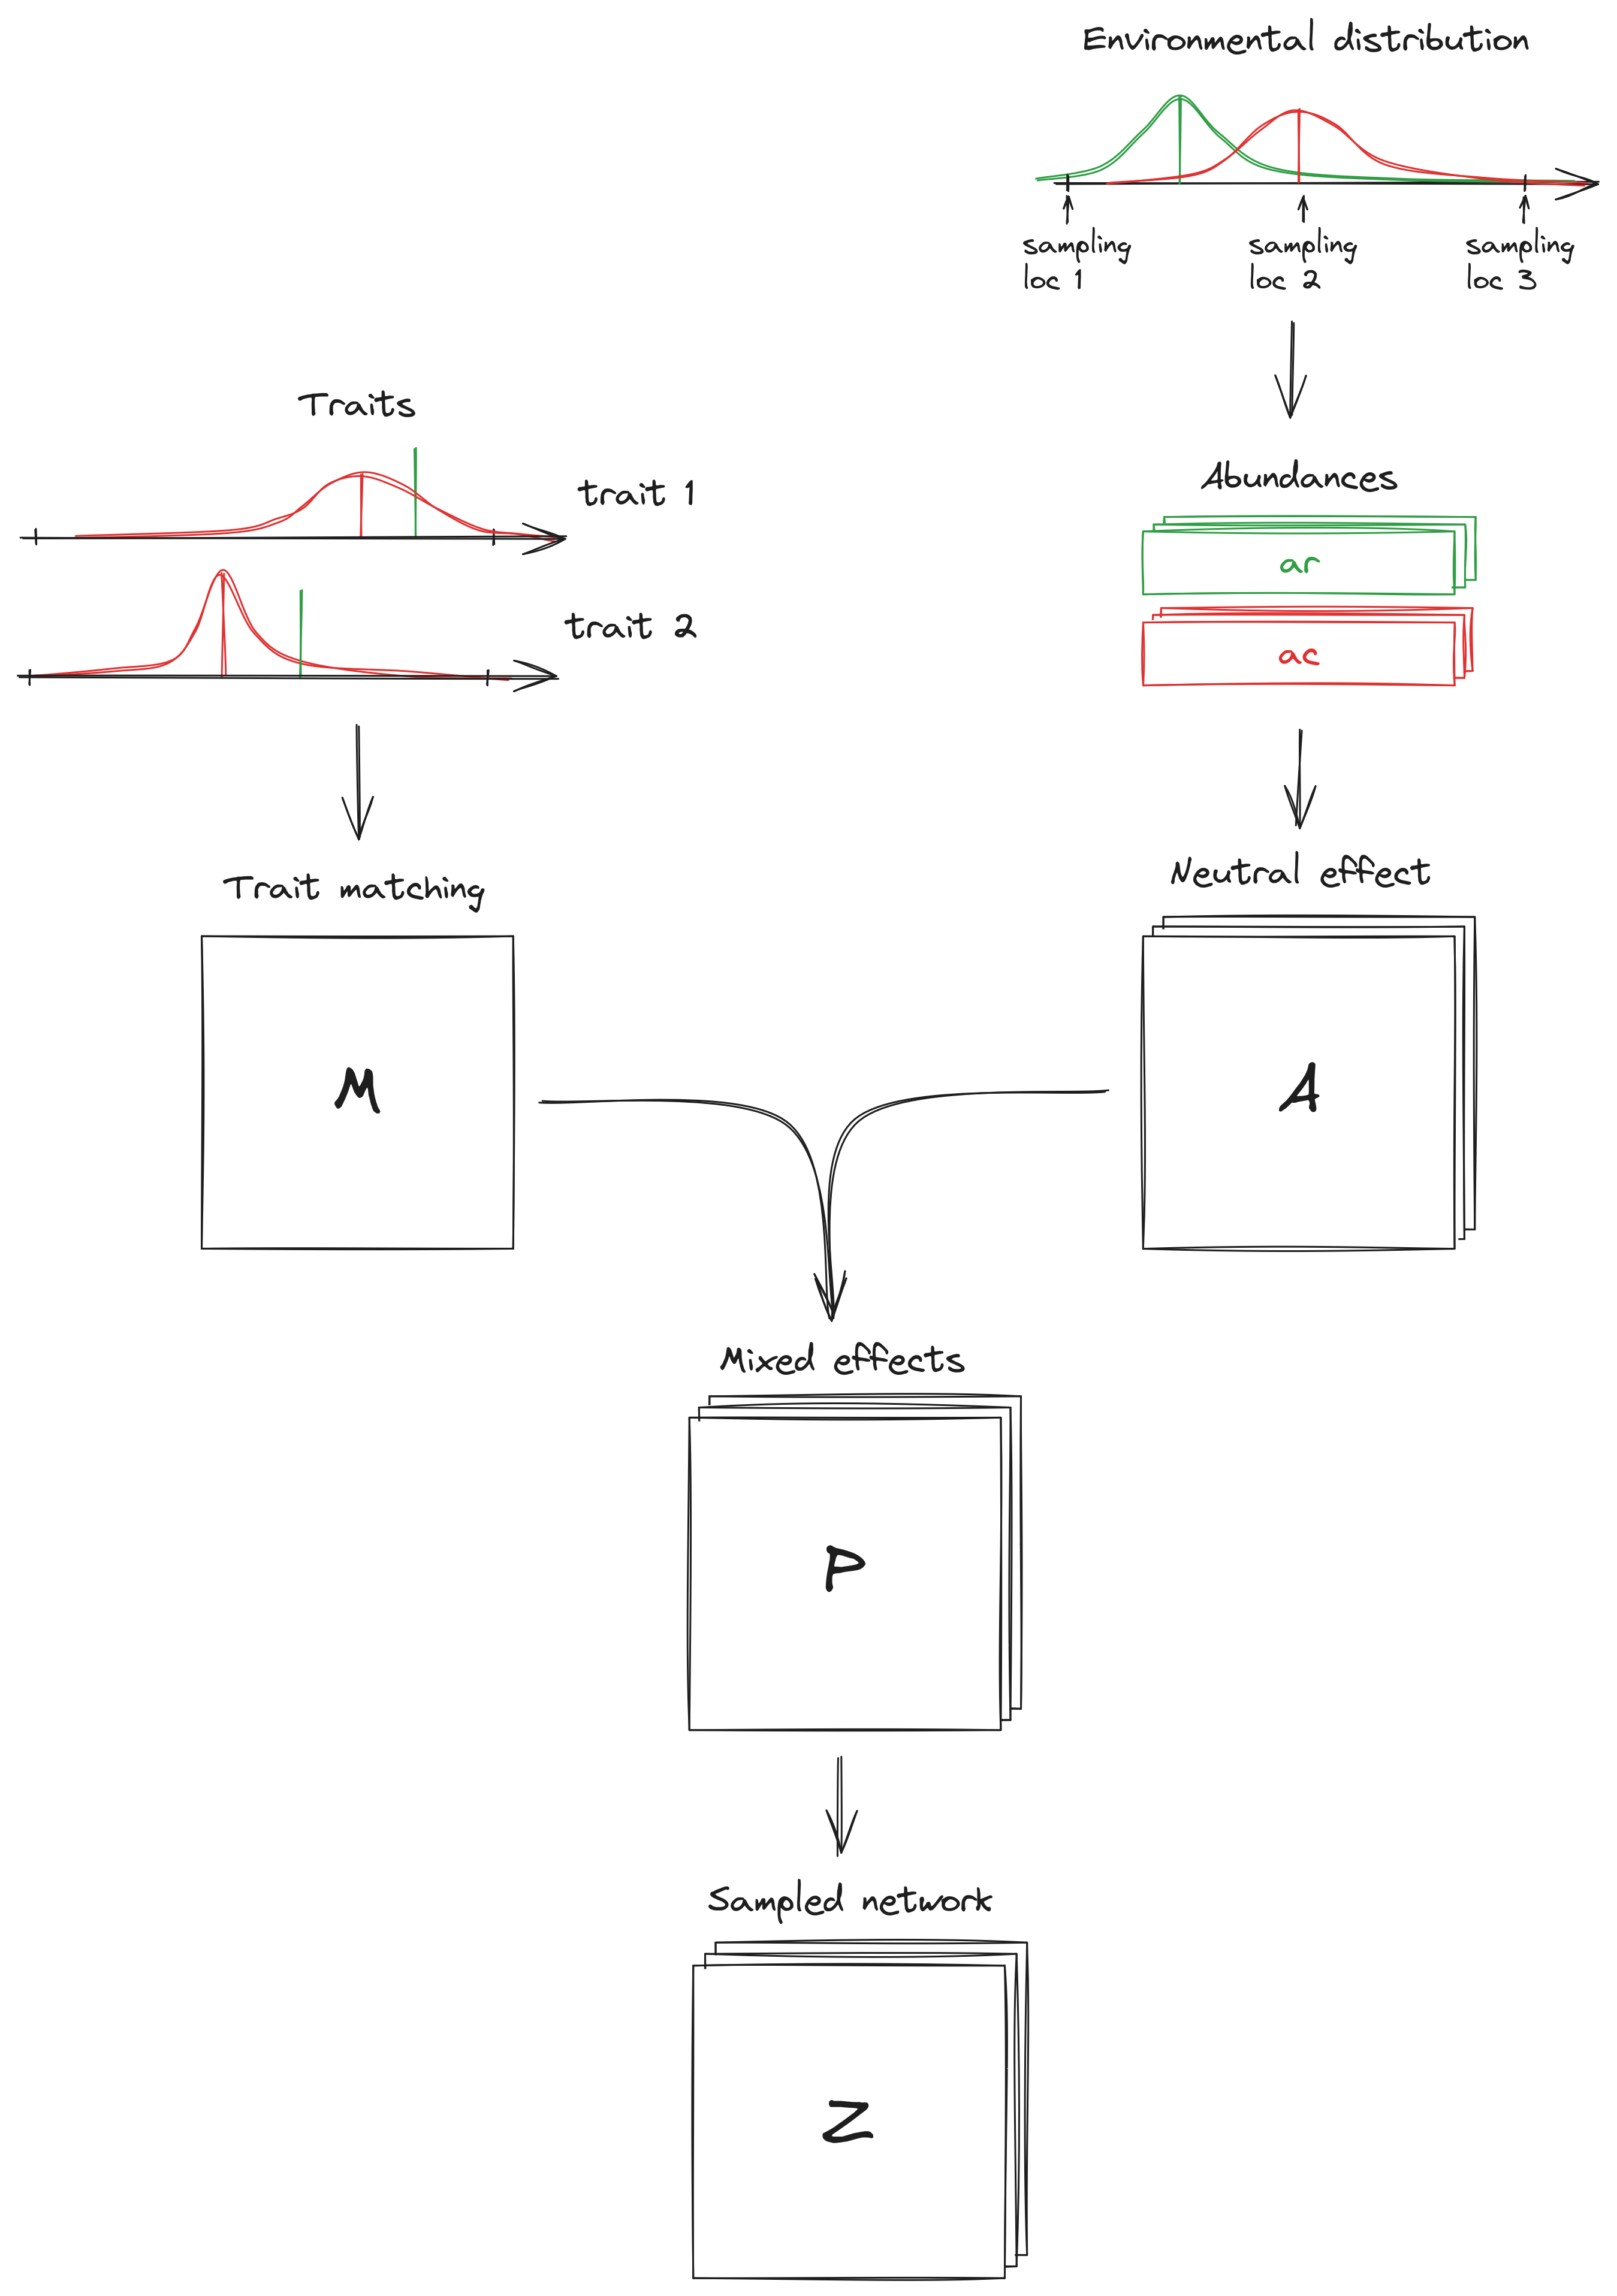
\includegraphics[width=0.8\linewidth]{FIGURES//methods/Netw_generation.png}
    \caption{Model steps used to simulate the interaction between consumer and resource species}
    \label{fig:netw_generation}
\end{figure}




\subsubsection{Traits generation}

Interactions are shaped by trait matching in ecosystems \citep{vazquez2009uniting}. To model these interactions, we need to generate traits for consumers and resources.


We simulate two traits for both the consumer and resource species. We define $\mathbf{T}^c = [t^c_{jk}]$ $(c \times 2)$ where $j$ is the number of consumer species and we similarly have $\mathbf{T}^r = [t^r_{ik}]$ $(r \times 2)$ where $i$ corresponds to the number of resource species.

The mean of the first trait is uniformly distributed between 0 and 1 for both consumers and resources. For the second trait, the span of the gradient is smaller such that it has a lesser driving weight on the matching.
For the consumer, each trait distribution is characterized by a mean (theoretical optimal trait value of the species) and a variance (indicating the degree of specialization or generalism) whereas for the resources there is only an optimum associated.

The trait matching does not have to be well-defined physical traits, such as the bill length or the fruit size. Traits can be a composite of multiple factors, including subjective ones like taste. For instance, the taste gradient of a fruit could range from sour/bitter to sweet. On the consumer side, the species would have a corresponding position to their taste and tolerance or intra-species variability.

The traits follow a normal distribution, with the means uniformly distributed between 0 and 1. The probability density function (PDF) for a resource with a trait $t_j$ and a consumer with an optimum at $t_i^r$ and a variance of $s_i^r$ is given by:

$$
    \mathbf{PDF:} \quad \frac{1}{\sigma_i\sqrt{2\pi}} exp -\left(\frac{t_j^c-t_i^r}{2s_i^r}\right)^{\!2}\
$$

\subsubsection{Interaction probability based on trait matching}

To compute the interaction probability solely based on trait matching, we assume that the interaction niche of the consumers follows a bivariate normal distribution defined by their traits. The likelihood of an interaction between a consumer and a resource to occur hence depends on the proximity of their optimums, which gives a notion of compatibility and tolerance of the consumer's trait.

Let $\mathbf{M} = [m_{ij}]$ be the trait-matching matrix, where $m_{ij}$ is the interaction probability between the consumer species $i$ and the resource $j$. This probability is given by:

$$
    \mathbf{M} = [m_{ij}]=\frac{1}{2\pi s_{j1}s_{j2}} exp\left(-\frac{(t^c_{j1} - t^r_{i1})^2}{2s^2_{j1}} - \frac{(t^c_{j2} - t^r_{i2})^2}{2s^2_{j2}}\right)
$$

where:
\begin{itemize}
    \item $t^r \text{ and }t^c$ are the traits optimums
    \item $s^2$ is the tolerance
\end{itemize}


\subsubsection{Abundances and environmental distribution}



In this section, we adopt the  Hutchinsonian definition of the environmental niche \citep{hutchinson_concluding_1957}, which describes a species as a position of the species in an $n$-dimensional gradient, in our case we set $n=1$ to keep the simulation simple.

We define an environmental gradient which can be interpreted as environmental factors such as humidity, soil resources availability, sun exposure, temperature, or the density of the environment. It could also represent time and hence seasonality fluctuations.

Similarly to the trait, each species is assigned a position and a tolerance on this environmental gradient that we will respectively call $\mathbf{E}^c = e_{jk}^c$ and $\mathbf{E}^r = e_{ik}^r$ for the consumers and resources.

To compute the number of individuals observed in a given quadrant during the observation time, we first compute the theoretical abundance of each species based on their position and a random factor, supposing that the niche distribution follows a Gaussian distribution.
The abundance $th\_a_{ix}$ of the species $i$ at the position $x$ on the gradient is given by:

$$
    th\_a_{ix} = N_i \cdot \frac{1}{\sigma_i\sqrt{2\pi}} exp \left( -\frac{(x-\mu_i)^2}{2\sigma_i^2} \right)
$$

where:
\begin{itemize}
    \item $N_i$ is a scaling factor representing the total population size proper to each species
    \item $x$ is the environmental position on the gradient
    \item $\mu_i$ is the niche optimum position of the species and $\sigma_i^2$ is the tolerance of the species
\end{itemize}

Then we simulate the vectors $a^c \text{ and } a^r$ containing the actual number of individuals observed during the sampling time using a Poisson process to take into account the stochasticity of the species presence. The observation count $a^c = [n_{ix}^c]$ for the species $i$ in the quadrat $x$ can be modeled as:

$$
    n_{ix}^c \thicksim Poisson(th\_a_{ix})
$$

\subsubsection{Interaction probability based on population size (neutral effect)}

We assume that the number of potential interactions in the network is proportional to the number of individuals, similar to how the speed of a reaction is proportional to the product of the reactant concentration. Therefore, we multiply the population size of consumers and resources for each network. 
Hence, we define the neutral effect matrix/ mean-field matrix $\mathbf{A}$ as : 

$$
    \mathbf{A} = [a_{ij}] = a^r a^{c\intercal}
$$

\subsubsection{Integration of trait matching and neutral effect}

The main assumption of this model is that species interactions are driven by both the relative abundance of the species and their compatibility regarding trait matching.

Depending on the weight given to trait-matching and neutral effect, we define the mixed effect probability matrix $\mathbf{P}$ as: 

$$
    \mathbf{P} = p^*_{ij} = \frac{{m_{i\mid j}}^\delta a_{ij}}{\sum_{i=1}^{r} \sum_{j=1}^{c}a_{ij}}
$$
    
where:
\begin{itemize}
\item  $\delta$ is a parameter that controls the weight given to trait matching compared to the neutral effect,
\item  $m_{i|j}$ represents the compatibility or matching score between species \(i\) and \(j\),
\item  $a_{ij}$ is the interaction term reflecting the relative abundance of species \(i\) and \(j\),
\item  $\sum_{i=1}^{r} \sum_{j=1}^{c}a_{ij}$ is a normalization constant ensuring that the elements of \(\mathbf{P}^*\) sum to 1.
\end{itemize}

The parameter $\delta$ allows the adjustment of the influence of trait matching in the model. When $\delta = 0$, the models rely only on the mean-filed (neutral) effect, meaning there are no preferences, and as $\delta$ increases, trait matching becomes the main driving factor of the interactions.



\subsubsection{Sampling of the interactions based on the previously computed probability}

To account for the bias in the sampling effort of the observed interaction, we sample $n_{inter}$ interactions using a multinomial distribution based on the probability matrix $\mathbf{P}$. The multinomial distribution with $\kappa = r \times c$ outcomes corresponds to the set of all the possible combinations of interactions.

The interaction counts are defined in the matrix $\mathbf{Z}$ as:

$$
    \mathbf{Z} \sim \mathcal{M}_{\kappa = rc}(n = n_\text{inter}, p = \mathbf{P})
$$

where:
\begin{itemize}
    \item $\mathbf{P}$ is the previously computed probability matrix of interactions,
    \item  $n_{\text{inter}}$ is the total number of sampled interactions,
    \item  $\mathcal{M}_{\kappa}$ denotes the multinomial distribution with \(\kappa\) possible outcomes.
\end{itemize}



\subsection{Reconstruction of latent traits}

To reconstruct the trait matching, we need to reverse the steps of the Correspondence Analysis (\ref{CA}). The same principle applies to the reconstruction of a Foucart CA as to the regular CA but we apply it to the aggregation of the different frames since the species' traits are supposed to be consistent across the frames.

First, we examine the distribution of the singular values and determine a cut-off on the number of axes to eliminate the noise.

Let $\mathbf{R}$ be the reconstruction for the first $k$ axes of the $\mathbf{C}$ matrix in the case of the multiples networks along an environmental gradient, or $\mathbf{S}$ if this is a single network. We define $\mathbf{R}$ as:
$$
    \mathbf{R} = \sum_{i=1} ^{k}\left( \mathbf{U}_{i,} \times \sigma_i \times \mathbf{V}_{i,}^\intercal \right)
$$

To retrieve the trait-matching matrix, we must remove the influence of abundance. We assumed that the number of interactions is proportional to the product of the relative abundances.  Thus, the best proxy for relative abundance are the rows and columns sums.

In CA, there is a normalization by the rows and columns sums. Thus, by reconstructing the matrix, we expect to retrieve the trait-matching matrix.

\subsection{Quantify trait matching}

In this section, we aim to quantify the performance of the Correspondence analysis in its ability to reconstruct the latent traits. We assume that the first axis is the proxy of the first trait and the second axis of the second trait. To do so, we look at the Pearson correlation coefficient between the theoretical trait given in input and the position. 

A perfect recovery of the trait is indicated by $\lvert cor(trait_{th}, position)\rvert = 1$, denoting a perfect linear relationship. Conversely, a complete absence of recovery would be $\lvert cor(trait_{th}, position)\rvert = 0$, signifying no linear relationship. 


\subsection{Research of reconstruction optimums}

The input parameters given to the simulation might unexpectedly impact the trait-matching performance. Therefore, we will look at the reconstruction performance between the first two traits and axes for different parameter values in a $50\times50$ network. The parameters we will focus on will be:
\begin{itemize}
    \item $n_{inter\_tot}$: the total number of observations across all the sampling sites,
    \item $n_{frames}$: the number of sampling sites,
    \item $\delta$: the weight given to trait matching as described in the simulation section (mettre une ref),
    \item $trait\_ratio$: the ratio between the amplitude of the first and the second trait,
    \item $\mu_{tol\_env}$: the mean of the environmental tolerance of both consumers and resources (the gradient ranges from 0 to 1),
    \item $\mu_{tol\_trait}$: the mean of the tolerance of the traits of the consumers (with the gradient ranging from 0 to 1).
\end{itemize}


\begin{table}[H]
    \centering
    \resizebox{\textwidth}{!}{%
    \begin{tabular}{c|c|c|c|c|c|c}
         Experiment&  $n_{inter\_tot}$ &  $n_{frames}$ &$\mu_{tol\_env}$ &  $\delta$&  $trait\_ratio$& $\mu_{tol\_trait}$\\
         \hline
         $n_{inter\_tot}$&  $250, 2500, 25000$&  5 &$0.5$&  $0.2$&  $0.7$& $0.1$\\
         $nb_{frames} \times \mu_{tol\_env}$&  $2500$&  $1,2,3,5,7,10$ &$0.1,0.3,0.5,0.7,1$&  $0.2$&  $0.7$& $0.1$\\
         $\delta$&  $2500$&  5 &$0.5$&  $0,0.01,0.1,0.2,1,2$&  $0.7$& $0.1$\\
         $trait\_ratio$&  $2500$&  $5$ &$0.5$&  $0.2$&  $0.1,0.3,0.5,0.7,0.9$& $0.1$\\
         $\mu_{tol\_trait}$&  $2500$&  $5$ &$0.5$&  $0.2$&  $0.7$& $0.01,0.005,0.1,0.2,0.3,0.5$\\
    \end{tabular}
    }
    \caption{Parameters for the experimentation}
    \label{parameter_table}
\end{table}



\subsection{Quantification of rewiring using Foucart COA}

Rewiring refers to the ability of species to change their interaction profile over time or in different environments. Using the Foucart Correspondence Analysis, we can obtain the positions of species in each sampling by projecting the corresponding network onto the same axes. CA positions the columns and rows with similar interaction profiles close to each other in the lower dimensional space.
We assume that the variance in the position of the CA is an estimator of the rewiring. As each position can be interpreted as a specific interaction profile., a high position's variance would imply a high diversity of the interaction profiles and hence a high level of rewiring.

\subsection{Beta diversity and interaction turnover}

Diverse ways can be used to describe a network. Historically, some of the most common metrics for bipartite ecological networks are connectance (the proportion of realized interactions over the ensemble of possible interactions), modularity (the degree to which edges are distributed within rather than between distinct sets of nodes), and link density (average number of links per node). While these metrics give a way to characterize a single network, they are limited when it comes to comparing networks among themselves.

Beta diversity, introduced by R.H. Whittaker \citep{whittaker_1960}, is an index ranging from 0 to 1 that measures the dissimilarity between two ecological communities. Let $A$ and $B$ be two realized communities. We define the beta diversity between these two communities as: 
$$
    \beta = \frac{a+b+c}{a+\frac{b}{2} + \frac{c}{2}} - 1
$$

where :
\begin{itemize}
    \item $a = ||A \cap B||$ is the number of species present in both communities,
    \item $b = ||B \notin A||$ is the number of species present only in the community $B$,
    \item $c = ||A \notin B||$ is the number of species present only in the community $A$.
\end{itemize}

Beta diversity can be extended in the context of ecological networks and broken down into two main different measures to quantify dissimilarity \citet{poisot_dissimilarity_2012}:
\begin{itemize}
    \item the dissimilarity in species composition ($\beta_S$), also called species turnover,
    \item the dissimilarity of interactions ($\beta_{WN}$).
\end{itemize}

 Interaction dissimilarity can be further decomposed into a dissimilarity of interactions due to species turnover ($\beta_{ST}$) and the dissimilarity of interactions due to the turnover of the links (turnover of the links within the set of species common to both networks, also called $\beta_{OS}$ or rewiring) such that $\beta_{WN} = \beta_{ST} + \beta_{OS}$. 

A recently published article by \citet{toju_interaction_2024} suggested a way to compute the species contribution to rewiring by removing each species one by one and computing the dissimilarity between the new $\beta_{OS,\Delta_i}$, and the original $\beta_{OS}$ as:
$$
    \Delta\beta_{OS,i} = \beta_{OS} - \beta_{OS,\Delta_i}
$$

\subsection{packages used}

All the computations and simulations were done on R (4.3.2), using ade4 (1.7-22) for the computation of Foucart Correspondence Analysis, ggplot2 (3.5.1) for data visualization part, and bipartite \citep{dormann_introducing_2008}(2.19) for beta diversity computation.
